\section{Automatic Accelerator Library Pre-building} \label{sec:lib-build}
 Accelerator library pre-building is essentially to pre-implement a group of SCGRA overlay based FPGA accelerators upon users' request. It is the basis for the proposed rapid FPGA loop accelerator generation framework. As QuickDough aims to enhance the designers' productivity and make FPGA accelerator design accessible to high-level application designers, the library pre-building process which involves low-level circuit design and optimization is thus automated so that it will not become a new barrier to the application developers. In this section, we will illustrate how the accelerator library is pre-built given the hardware resource budget and target loop kernels.

\figref{fig:auto-lib-gen} presents the proposed 4-step automatic accelerator library pre-building flow. Given a group of high-level loop kernels to be accelerated using QuickDough, it extracts DFGs from the loop kernels first by using the DFG generator. Afterwards, operation sets that are needed for each loop kernel can be decided. By utilizing an operation set similarity metric, the loop kernels are divided into different clusters in the second step. Basically, loop kernels that require a similar operation set are considered as the same cluster and therefore corresponding accelerator library will be pre-built for each cluster of applications in next steps. After the loop kernel classification, a representative accelerator configurations will be generated for each cluster of loop kernels based on the SCGRA overlay template and the resource constraints in the third step. Finally, the accelerator libraries to be built will be implemented on a parallel computing machine. Since DFG generation has been discussed in previous section, we will mainly detail the rest three steps in this section.

\begin{figure}
\vspace{-1em}
    \center{\includegraphics[width=0.5\linewidth]{lib-gen}}
\caption{Automatic SCGRA overlay based FPGA accelerator library update}
\label{fig:auto-lib-gen}
\vspace{-1.5em}
\end{figure}

\subsection{Common operation analysis}
As mentioned in previous sub section, the common operation analysis step first divides the loop kernels into different clusters based on the operation set similarity between the loop kernels and then generates a common operation set for each cluster of applications. 

In this work, we use Jaccard coefficient as the similarity metric. Suppose there are $N$ loop kernels to be analyzed, $C_i$ and $C_j$ are the operation sets of two loop kernels where $i,j=1,2,...,N$. Then the Jaccard coefficient of any two loop kernels $S_{ij}$ can be calculated using \eqnref{eq:jaccard}. 

\begin{equation} \label{eq:jaccard}
S_{ij}=\frac{C_i \cap C_j}{C_i \cup C_j}
\end{equation}

As some of the operations can be complex and consume a lot of hardware resource, it may be better to build separate library for loop kernels that only differ on such an operation. To that end, we may also take the overhead of the operations into consideration while calculating the similarity coefficient. Assume $IW_{ij}$ and $UW_{ij}$ as weight vectors of operations in $C_i \cap C_j$ and $C_j \cup C_j$ respectively, and then the similarity matrix of the loop kernels can be calculated using \eqnref{eq:wjaccard} instead.  

\begin{equation} \label{eq:wjaccard}
S_{ij}=\frac{\sum\nolimits(IW_{ij})}{\sum\nolimits(UW_{ij})}
\end{equation}

When the similarity matrix of the target loop kernels are obtained, a user specified threshold $T$ is used to decide whether the two loops can be considered as a cluster. According to the definition, $S_{ij}$ is close to 1 when two operation sets are similar. Thus when $S_{ij} \ge T$, the two loop kernels can be put in the same cluster. Otherwise, they will be divided into separate clusters.

When the loop kernels are divided into different clusters, we can further obtain the minimum common operation set of each cluster of loop kernels, which is essentially a union of the operation sets included in the loop kernels of the same cluster. The analysis is trivial, but the minimum operation set can be decided automatically and rapidly.

\subsection{Minimum accelerator configuration set analysis}
Although the library can be implemented off-line, it does take a long time to complete. Therefore, we try to find out the minimum set of accelerator configurations that need to be pre-implemented as the library for each cluster of loop kernels and maintain the application coverage of the library at the same time. 

The proposed SCGRA overlay based FPGA accelerator utilizes block RAM to implement the instruction memory, data memory, on-chip buffer as well as the address buffer, and block RAM is the hardware resource bottleneck. As a result, the library basically depends on how the block RAM budget is allocated to different components of the accelerators. Therefore, the minimum library can be obtained using equation \eqnref{eq:lib-gen}. $Row$ and $Col$ stand for the SCGRA overlay size and they are integers. $IM$, $DM$, $AIOB$ and $DIOB$ stand for the instruction memory capacity, data memory capacity, address IO buffer capacity and IO buffer capacity. In addition, they can only increase with the granularity of a primitive block RAM. $B$ stands for the user specified block RAM budget. 

\begin{equation} \label{eq:lib-gen}
    \footnotesize
    Row \times Col \times(IM + DM) + AIOB + IOB \leq B
\end{equation}

Moreover, empirical settings such as limiting data memory in each PE to a single primitive block RAM
(i.e. $DM = 1$), constraining the difference between SCGRA row size and column size (i.e. $Col \leq
Row \leq (Col + Gap)$, $Gap$ is an integer) and setting $AIOB = IOB$ are employed to further reduce the number of
accelerators pre-built in the library. Meanwhile, the accelerator configurations to be built are also determined.

\subsection{Accelerator HDL model generation and implementation}
With the proposed SCGRA overlay template and the required operation set, ALU data path will be updated first. Currently, the data paths of the ALU are manually created, but it is possible to rely on the high level synthesis tools in future. Then HDL models of the accelerators can be generated based on the configurations decided in the third step. This part is done with a python script. 

When all the HDL codes of the accelerators are generated, they can be further implemented using the classical hardware implementation tools. As the implementation jobs are completely independent, they can be done in parallel on either a multi-core processor or a cluster conveniently. Moreover, the regular tiling structure even allows the implementations to be accelerated using macro based implementation techniques as presented in \cite{ROB2015}, which can be up to 20X faster than a standard HDL implementation with negligible timing and overhead penalty. After the implementation, implementation frequency is added to the corresponding accelerator configuration, which completes the whole library generation process.
